%\documentstyle[epsf,twocolumn]{jarticle}       %LaTeX2e仕様
\documentclass[twocolumn]{jarticle}     %pLaTeX2e仕様(platex.exeの場合)
% \documentclass[onecolumn]{ujarticle}   %pLaTeX2e仕様(uplatex.exeの場合)
%%%%%%%%%%%%%%%%%%%%%%%%%%%%%%%%%%%%%%%%%%%%%%%%%%%%%%%%%%%%%%
%%
%%  基本バージョン
%%
%%%%%%%%%%%%%%%%%%%%%%%%%%%%%%%%%%%%%%%%%%%%%%%%%%%%%%%%%%%%%%%%
\setlength{\topmargin}{-45pt}
%\setlength{\oddsidemargin}{0cm}
\setlength{\oddsidemargin}{-7.5mm}
%\setlength{\evensidemargin}{0cm}
\setlength{\textheight}{24.1cm}
%setlength{\textheight}{25cm}
\setlength{\textwidth}{17.4cm}
%\setlength{\textwidth}{172mm}
\setlength{\columnsep}{11mm}

%\kanjiskip=.07zw plus.5pt minus.5pt


% 【節が変わるごとに (1.1)(1.2) … (2.1)(2.2) と数式番号をつけるとき】
%\makeatletter
%\renewcommand{\theequation}{%
%\thesection.\arabic{equation}} %\@addtoreset{equation}{section}
%\makeatother

%\renewcommand{\arraystretch}{0.95} 行間の設定
%%%%%%%%%%%%%%%%%%%%%%%%%%%%%%%%%%%%%%%%%%%%%%%%%%%%%%%%
%\usepackage{graphicx}   %pLaTeX2e仕様(\documentstyle ->\documentclass)
\usepackage[dvipdfmx]{graphicx}
\usepackage{subcaption}
\usepackage{multirow}
\usepackage{amsmath}
\usepackage{url}
\usepackage{ulem}
\usepackage{algorithm}
\usepackage{algorithmic}
\usepackage{listings} %,jlisting} %日本語のコメントアウトをする場合jlistingが必要
%ここからソースコードの表示に関する設定
\lstset{
  basicstyle={\ttfamily},
  identifierstyle={\small},
  commentstyle={\smallitshape},
  keywordstyle={\small\bfseries},
  ndkeywordstyle={\small},
  stringstyle={\small\ttfamily},
  frame={tb},
  breaklines=true,
  columns=[l]{fullflexible},
  numbers=left,
  xrightmargin=0zw,
  xleftmargin=3zw,
  numberstyle={\scriptsize},
  stepnumber=1,
  numbersep=1zw,
  lineskip=-0.5ex
}
%%%%%%%%%%%%%%%%%%%%%%%%%%%%%%%%%%%%%%%%%%%%%%%%%%%%%%%%
\begin{document}

	%bibtex用の設定
	%\bibliographystyle{ujarticle}

	\twocolumn[
		\noindent
		\hspace{1em}
		後期研究発表会資料 2020 年 12 月 14 日 (月)
		\hfill
		B4 杉山 竜弥
		\vspace{2mm}

		\hrule
		\begin{center}
			{\Large \bf DARTSを用いたVGGのショートカット探索とGAによる改良}
		\end{center}
		\hrule
		\vspace{9mm}
	]

\section{はじめに}
機械学習の分野では, 深層学習モデルの改良によって高い精度を得てきた.
しかしモデルの設計とその性能の関係はブラックボックスであり
手作業で行うチューニングには膨大な労力を要する.

ネットワークの探索を自動化する手法として提案された
Neural Architecture Search(NAS)はネットワークを機械学習によって探索する.
しかし何千ものGPUを必要とするため, NASに代わり
小規模な資源で計算できるDifferentiable Architecture Search(DARTS)
が大きな注目を集めている.
DARTSはネットワークの構造と演算子の候補を探索するが,
一方でDARTSにはネットワーク構造にいくつかの拘束条件がある.

本研究では演算子の種類ではなくネットワークの構造にのみ着目し,
DARTSの構造制限をなくしネットワークの柔軟な探索を目的とする.
その初期段階として, VGGのショートカット位置についてDARTSで探索を行う方法を提案する.

\section{要素技術}

\subsection{Neural Architecture Search}
Neural Architecture Search(NAS)\cite{DBLP:journals/corr/ZophL16}は,
機械学習の分野で使用されているニューラルネットワークの設計を自動化する手法である.
ニューラルネットワークの設計は直感的でなく,
チューニングに人による労力を多く必要とするため,
ニューラルネットワークの設計は非常に困難である.

NASはニューラルネットワークが構造に関する設定の文字列で表現できることを利用して,
この文字列を生成する
Recurrent Neural Network(RNN)を
強化学習 Reinforcement Learning(RL)によって学習する.
% RNNによって生成されたアーキテクチャは, 検証データで性能評価され

\subsection{Differentiable Architecture Search}
Differentiable Architecture Search(DARTS)\cite{DBLP:journals/corr/abs-1806-09055}は,
離散的なアーキテクチャ探索空間に強化学習を適用したNASとは異なり,
微分可能な方法で定式化し,
偏微分による勾配降下法を使用してアーキテクチャを効率的に探索する手法である.

探索空間を連続にするため, カテゴリカルな演算子の選択の代わりに, 候補全ての可能性をもつ混合演算子を
(\ref{eq:darts/operation}) 式で定義する.
アーキテクチャを有向非巡回グラフで表したとき, ノードを潜在的な特徴表現 $x^{(i)}$,
エッジを特徴 $x^{(i)}$ が適用される関数 $o(・)$ とすると,
\begin{equation}
  \label{eq:darts/operation}
  \bar{o}^{(i, j)}(x) = \sum_{o \in \mathcal{O}} \frac{\exp(\alpha^{(i, j)}_o)}{\sum_{o' \in \mathcal{O}} \exp(\alpha^{(i, j)}_{o'})} o(x)
\end{equation}
となる. ここで
$\mathcal{O}$ は探索する演算子の候補集合,
$\alpha^{(i, j)}$ はエッジ $(i, j)$ の混合演算子の重みベクトルである.
DARTSは勾配降下法によって連続変数集合$\alpha$を学習する.

$\alpha$ とレイヤーの重み $w$ のBi-Level最適化問題を $w$ の近似によって同時に学習し,
NASの3000 GPU daysに対してDARTSは3.3 GPU daysに高速化した.

DARTSでは次元を統一するためセルと呼ぶ小さなネットワーク構造を重ねたモデルを利用する.
セルを構成するノードは2つのノードからの演算子エッジを持ち,
どのノードからの演算子を選ぶのかをアーキテクチャを示す重み $\alpha$ によって決定する.
DARTSの問題点として位置と演算子の種類は探索できるが,
大局的な構造やノードの持つエッジ数などアーキテクチャが固定されていることが挙げられる.

% セルとノードの関係を図示してもいい(DARTSのやつ)

\subsection{Genetic Algorithm}
遺伝的アルゴリズム(Genetic Algorithm : GA)は生物の進化の仕組みを模倣した最適化手法である.
問題の解候補を遺伝子の持つ個体として表現し, 適応度によって個体を評価・選択する.
交叉・突然変異などの操作によって解候補の多様性を保ちつつ,
近傍を探索しながら世代を重ねて近似的な最適解を求める.
% GAに必要な条件は評価関数の全順序性と探索空間が位相を持つことである.

% 整数値と実数値

% 初期収束問題
GAには偶然適応度の高くなった個体だけが選択され続け,
個体群を同じ個体が占める初期収束問題がある.
問題によって適切な交叉・突然変異を行う必要がある.

\section{問題}
% 問題・探索空間
DARTSで柔軟なアーキテクチャを探索するため,
深層畳み込みネットワークのVGG19\cite{Simonyan15}のショートカット接続を探索する.
VGG19は16層の畳み込み層と3層の線形結合層を持つ.
このVGG19に対し層を飛ばして接続するショートカットの数と位置を求め,
性能を向上させることを目的とする.

モデル中の潜在的特徴は高さ・幅・チャンネル数を持つデータであるが,
特徴の次元は場所によって異なるため, ショートカットは次元を変換する必要がある.
したがってショートカット関数は以下のように設定した.
\begin{enumerate}
  \item 次元が同じ場合:恒等関数
  \item フィルタ数が違う場合:Pointwise Convolution
  \item 高さと幅が半分の場合:Factorized Reduce
  \item それ以外の場合:ショートカットを定義しない
\end{enumerate}
ショートカットに使用する関数の制限によってショートカット位置の候補は61であるため,
探索空間は$2^{61}$である.
演算子の種類は固定することで, アーキテクチャ $\alpha$ は畳み込み部に相当するグラフの重みをもつ隣接行列と定義した.

\section{手法と実験1}
% アルゴリズム

ショートカットの本数も探索するため,
$\alpha$ に対する重み補正 $\beta$ を (\ref{equ:cut}) 式 で定義する.
\begin{equation}
  \label{equ:cut}
  x_i = f^{\mathrm{c}}_{i-1, i}(x_{i-1}) + \beta_i * \sum_{j \in S_i} \alpha_{ij} * f^{\mathrm{s}}_{j, i} (x_j)
\end{equation}
ここで $f^{\mathrm{c}}(・)$, $f^{\mathrm{s}}(・)$ は, VGGの畳み込み関数とショートカット関数,
$S_i$ はノード $i$ とショートカットで接続する先行(predecessor)ノードのインデックス集合である.

ただし$\beta=0$で勾配の更新ができなくなるので,
\begin{equation}
  \label{equ:beta}
  \hat{\beta} = \begin{cases}
    \exp(\beta - 1) & (\beta \leq 1) \\
    \log(\beta) + 1 & (\mathrm{otherwise})
  \end{cases}
\end{equation}
で0とならないように補正した $\hat{\beta}$ を用いた.

学習の手順は以下.
\begin{enumerate}
  \item 探索:アーキテクチャ $\alpha$ の訓練
  \item 構成:$\alpha$ からネットワークを構成
  \item 評価:得られたネットワークを訓練し, テストデータで性能を評価
\end{enumerate}

構成手法は複数考えられるため,
\begin{itemize}
  \item 構成手法A:predecessorsの中で大きい順に採択
  \item 構成手法B:閾値以上のエッジを採択
\end{itemize}
で実験した.

\subsection{実験設定}

\begin{table}[tb]
  \begin{center}
    \caption{実験1の設定}
    \begin{tabular}{|c|c|} \hline
      Loss & Cross Entropy Loss \\ \hline
      batch size & 64 \\ \hline\hline
      Step & Architecture Search \\ \hline
      Optim($w$) & SGD(lr=0.001, momentum=0.9) \\ \hline
      Optim($\alpha$) & Adam(lr=0.003, $\beta$=(0.5, 0.999)) \\ \hline
      data size & train : valid : test = 25000 : 25000 : 10000\\ \hline\hline
      Step & Evaluation \\ \hline
      Optim($w$) & SGD(lr=0.0090131, momentum=0.9) \\ \hline
      Scheduler($w$) & Step($\gamma$=0.23440, stepsize=100) \\ \hline
      data size & train : valid : test = 50000 : 0 : 10000\\ \hline
    \end{tabular}
    \label{tab:setting1}
  \end{center}
\end{table}

表 \ref{tab:setting1} に探索段階と評価段階の実験設定を示す.
探索段階はDARTSを参考に, 評価段階はoptunaで最適化した値を使用した.

データセットは, 訓練画像が 32 pixel 四方で訓練データを50000枚持つ CIFAR-10 を利用して,
10クラス分類問題を解いた.

探索時間は, 150 epochとし, 50 epochごとにその時点の $\alpha$ の性能を評価した.

構成段階では手法A, Bに加えて比較のため,
ショートカット数が同じとなる条件でランダムに選択する手法でも実験する.
各手法において10回試行して統計的な性能を比較した.

\subsection{結果}

\begin{table*}[t]
  \begin{center}
    \caption{各アーキテクチャの精度}
    \begin{tabular}{|c|c|c|c|c|c|}\hline
    \multicolumn{2}{|c|}{\textbf{architecture}} & \textbf{\begin{tabular}[c]{@{}c@{}}test accuracy\\ (\%)\end{tabular}} & \textbf{\begin{tabular}[c]{@{}c@{}}param\\ (M)\end{tabular}} & \textbf{\begin{tabular}[c]{@{}c@{}}number of\\ shortcuts\end{tabular}} & \textbf{\begin{tabular}[c]{@{}c@{}}random architect\\ accuracy (\%)\end{tabular}} \\ \hline
    \multirow{3}{*}{\begin{tabular}[c]{@{}c@{}}method A\end{tabular}} & 50 epoch & 93.70 $\pm$ 0.22 & 21.06 $\pm$ 0.07 & 12.7 $\pm$ 1.4 & 93.60 $\pm$ 0.15 \\ \cline{2-6}
     & 100 epoch & 94.02 $\pm$ 0.12 & 21.50 $\pm$ 0.11 & 18.2 $\pm$ 0.9 & 93.67 $\pm$ 0.14 \\ \cline{2-6}
     & 150 epoch & 93.90 $\pm$ 0.17 & 21.57 $\pm$ 0.25 & 18.9 $\pm$ 0.6 & 93.64 $\pm$ 0.09 \\ \hline
    \multirow{3}{*}{\begin{tabular}[c]{@{}c@{}}method B\end{tabular}} & 50 epoch & 93.57 $\pm$ 0.19 & 20.45 $\pm$ 0.09 & 5.8 $\pm$ 1.2 & 93.36 $\pm$ 0.19 \\ \cline{2-6}
     & 100 epoch & 93.93 $\pm$ 0.08 & 20.73 $\pm$ 0.10 & 9.8 $\pm$ 1.0 & 93.47 $\pm$ 0.17 \\ \cline{2-6}
     & 150 epoch & 93.92 $\pm$ 0.12 & 20.76 $\pm$ 0.15 & 10.6 $\pm$ 1.0 & 93.48 $\pm$ 0.15 \\ \hline
    \multicolumn{2}{|c|}{baseline (VGG19)} & 93.03 $\pm$ 0.10 & 20.04 & 0 & - \\ \hline
    \end{tabular}
    \label{tab:accg}
  \end{center}
\end{table*}

\begin{figure*}[tb]
 \begin{minipage}{0.5\hsize}
 	\begin{center}
 		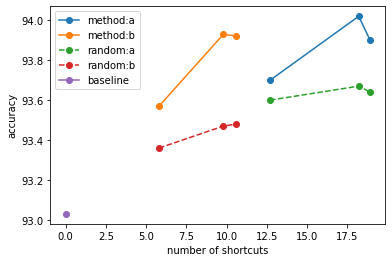
\includegraphics[clip,width=75mm]{short.png}
 		\caption{ショートカット数に対する精度}
 		\label{fig:short}
 	\end{center}
 \end{minipage}
 \begin{minipage}{0.5\hsize}
 	\begin{center}
    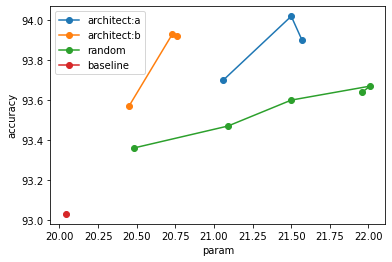
\includegraphics[clip,width=75mm]{param.png}
    \caption{パラメータ数に対する精度}
    \label{fig:param}
 	\end{center}
 \end{minipage}
\end{figure*}


表 \ref{tab:accg} に各構成手法におけるテストデータの精度を示す.
図 \ref{fig:short}, \ref{fig:param} には
表 \ref{tab:accg} の精度に対するショートカット数とパラメータ数の関係を図示する.
最も性能が高かったのは100 epoch 時点の手法Aで94.02 \%(baseline+0.99\%)となり,
100 epoch 時点の手法Bは93.93 \%(baseline+0.90\%)となった.
しかしランダム手法と比較すると, 手法Aは+0.35\%, 手法Bは+0.46\%となり,
図 \ref{fig:param} を参照しても少ないパラメータ数でより有効に探索できているのは手法Bと言える.

また100 epoch時点と150 epoch時点を比較すると, 学習によって性能が悪化している.
問題に対して過度に適合していることが原因であると考えられる.

探索時間は150 epochでおよそ 5 gpu hours を要したが, DARTSと比べ演算子の探索を行っていないことや.
最適な重み $w^*$ の近似を1次下げていることで高速になったと思われる.




\section{手法と実験2(GA)}
実験1では $\alpha$ の学習度によって重み $w$ の学習しやすさに偏りがあったため,
収束するグラフ構造にばらつきが見られた.

そこで個体表現を $\alpha$ とした遺伝的アルゴリズムによって,
アーキテクチャの多様性を維持しつつ, 安定的な
ネットワーク構造の学習を図った.

% GAには評価関数の全順序性が必要となるので,(これは間違い)
各パラメータ集合の学習ステップを分離し個体間で不平等がないように設計した.

\begin{enumerate}
  \item 一様乱数で初期個体生成
  % \item 重み$w$を$\displaystyle \sum_{i \in P} \nabla_w \mathcal{L}_{\mathrm{train}}(w^*, \alpha^\mathrm{sampled}_i)$で更新
  \item 重み $w$ を $\displaystyle \nabla_w \mathcal{L}_{\mathrm{train}}(w^*, \bar{\alpha})$ で更新
  \item 個体 $\alpha_i$ を $\displaystyle \nabla_\alpha \mathcal{L}_{\mathrm{valid}}(w^*, \alpha_i)$ で更新
  \item 適応度 $\displaystyle \mathcal{L}_{\mathrm{test}}(w, \alpha^\mathrm{sampled})$ で個体 $\alpha$ を評価・選択
  \item 交叉・突然変異
  \item 収束するまで 2. に戻る
\end{enumerate}
ただし
% $P$は個体群,
$\bar{\alpha}$ は各個体の平均,
$\alpha^\mathrm{sampled}$ は構成手法Bで隣接行列にサンプリングした $\alpha$ .

学習後最終世代の個体の性能を実験1と同じ条件で評価した.

\subsection{実験設定}

表 \ref{tab:setting2}, \ref{tab:setting_ga}にモデルとGAの実験設定を示した.
モデルの重み $w$ はImage Netで訓練された事前学習の重みを畳み込み層の部分に適用した.
初期収束を防ぐため, 交叉にはエッジに相当する遺伝子座ごとに 0.5 の確率で操作する一様交叉を使用した.
突然変異には遺伝子座ごとに 0.1 の確率で $\mu=0$, $\gamma=0.2$ となるガウス分布からの摂動を与えた.


\begin{table}[t]
  \begin{center}
    \caption{実験2の設定}
    \begin{tabular}{|c|c|} \hline
      Optim($w$) & SGD(lr=0.001, momentum=0.9) \\ \hline
      Optim($\alpha$) & Adam(lr=0.003, $\beta$=(0.5, 0.999)) \\ \hline
      Loss & Cross Entropy Loss \\ \hline
      pretrain & true \\ \hline
      batch size & 64 \\ \hline
      train size & 25000 \\ \hline
      valid size & 10000 \\ \hline
    \end{tabular}
    \label{tab:setting2}
  \end{center}
\end{table}

\begin{table}[t]
  \begin{center}
    \caption{GAの設定}
    \begin{tabular}{|c|c|} \hline
      個体数 & 15 \\ \hline
      世代数 & 20 \\ \hline \hline
      選択 & トーナメント \\ \hline
      サイズ & 2 \\ \hline \hline
      交叉 & 一様交叉 \\ \hline
      交叉率 & 0.8 \\ \hline \hline
      変異 & ガウス分布 \\ \hline
      変異率 & 0.2 \\ \hline
    \end{tabular}
    \label{tab:setting_ga}
  \end{center}
\end{table}

% 表 \ref{tab:setting}, \ref{tab:setting_ga} にモデルとGAの設定を示した.
% 初期収束を回避するため, トーナメントサイズや交叉アルゴリズムを変更した.

\subsection{結果}
図 \ref{fig:gene_acc}

\begin{figure}[tb]
  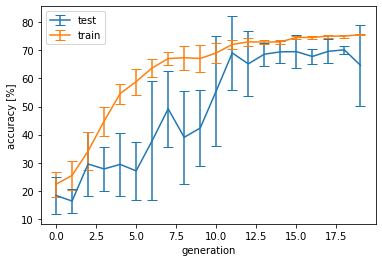
\includegraphics[clip, width=75mm]{acc.png}
  \caption{世代ごとの精度}
  \label{fig:gene_acc}
\end{figure}

\section{まとめと今後の課題}
% なんとなくなんかの勉強をするとかではなく具体的に
DARTSの欠点であるアーキテクチャ構造の制限を緩和するようなネットワーク探索ができた.

ネットワークの構成手法は改善の余地がある.
選択しないという候補を導入して, 他のショートカットと妥当な比較ができると考えられる.

GAを導入することでショートカットの本数の分析もできた.

他のデータセットや実問題に対して提案手法によるアーキテクチャの汎用性を確認したい.

% 参考文献リスト
\bibliographystyle{unsrt}
\bibliography{ref}
\end{document}
